
\newglossaryentry{X}
{
  type=differential-privacy,
  name={$\ensuremath{X} $},
  description={Set of locations for a user. ($R^2$)},
}
\newglossaryentry{Z}
{
  type=differential-privacy,
  name={$\ensuremath{Z} $},
  description={For every $x \in X$ a perturbed location $z \in Z$ is reported.},
}
\newglossaryentry{K}
{
  type=differential-privacy,
  name={$K(x)(Z)$},
  description={Randomization method for $x \in X$ and output $z \in Z$.},
}
\newglossaryentry{Epsilon}
{
  type=differential-privacy,
  name={$\ensuremath{\epsilon} $},
  description={The privacy budget $\epsilon$ determines the amount of noise that is added.
    },
}
\newglossaryentry{Pr}{
  type=differential-privacy,
  name={$Pr(K(x_i) \in (Z))$},
  description={Probability of reporting $x \in X$ for $z \in Z$}
}


\section{Differential privacy} \label{section:dp}
\todo[inline]{Explain general notion of privacy}
\glsaddall
\leading{10pt}
\printglossary[type=differential-privacy, nonumberlist]
\begin{figure}[h]
  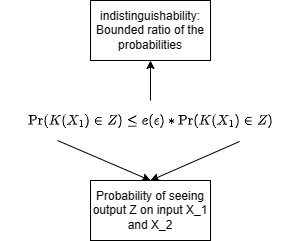
\includegraphics{TheorethicalFramework/Differential privacy/master-thesis-Differential privacy illustration.png}
  \caption{Randomization function $K$ gives $\epsilon$-differential privacy for all elements in $D_1$ and $D_2$ if they differ at most one element. \citep{dwork_differential_2006}}
  \label{fig:definition-dp}
\end{figure}
The privacy budget $\epsilon$ determines the amount of noise that is added.
\subsection{Laplace algorithm}
One way to achieve $\epsilon$-DP is using sampling noise from the Laplace or Gaussian distributions.
\todo[inline]{Explain Gaussian / Laplace distributions}
The noise is then based on the sensitivity of a function $f$.
This is the maximal possible change when adding or removing a single record \citep{friedman_data_2010, dwork_differential_2006}.
\begin{equation}
  \Delta f = max_{D_1, D_2} ||f(D_1) - f(D_2)||
\end{equation}
% This means, that if the sensitivity is low, the noise is as well.
% The metric is combined with the privacy budget $\epsilon$ to control the noise that is being added by a mechanism like Laplace \citep{friedman_data_2010}.
\todo[inline]{Explain differential privacy implementation with La place distribution}



\subsection{Local differential privacy}
\subsection{Geo-indistinguishability}

%The above attacks mainly target the clustering method after they have been trained. 
%$Various attacks are more focused on data, like 
%\subsection{Evaluation methods} \label{theory:evaluation-dp}
\mycomment{
  It is possible to evaluate and measure the impact of the noise between two distributions by calculating the error between the non-private and private data \citep{del_rey_comprehensive_2020-1}.
  Two metrics that are proposed by the same study are Mean Squared Error (MSE) and Mean Average Error (MAE).
  These metrics can be used to calculate the error between $X$ and the perturbed dataset $Z$. \newline

  Just as it is possible to measure the utility, this can also be done with privacy.
  When performing a privacy algorithm, it can be proven whether a method meets the privacy requirements.
  These are metrics such as $\epsilon$-differential-privacy (\ref{fig:definition-dp}) and $\epsilon$-geo-indistinguishability (see next chapter \ref{algo:2d-geo-indistinguishability}).
  Although these methods give an idea of privacy, it can only be "yes" or "no".
  Furthermore, it can give a distorted image, since a chance of 70\% also gives a "yes" according to the definition of geo-indistinguishability \citep{oya_is_2017}.
  In other words, to gain more insight into the amount of privacy (such as with MSE or MAE), other metrics are needed.

  For this reason, Oya et al. introduced a metric for geo-indistinguishability that makes it possible to give percentages in their study \citep{oya_is_2017}:
  As an example, an adversary is given that guesses between two locations: $x \in X$ and  $x' \in X$.
  \begin{equation}
    p_e (x, x', z) \leq p^*_e = \frac{1}{1 + e^{e * d(x, x')}}
    \label{eq:geo-as-an-error}
  \end{equation}
  Where privacy level $p^*_e$ is the lower bound of the probability of an adversary guessing correctly.
  The method is called $\epsilon$-geo-indistinguishability as error.
  Based on this metric, it can be calculated that an adversary has an average of 90\% chance to guess a location correctly.
  In that case, the algorithm would be $\epsilon$-geo-indistinguishability, but in practice not.
}